\documentclass[conference]{IEEEtran}
\IEEEoverridecommandlockouts
% The preceding line is only needed to identify funding in the first footnote. If that is unneeded, please comment it out.
\makeatletter
\def\endthebibliography{%
	\def\@noitemerr{\@latex@warning{Empty `thebibliography' environment}}%
	\endlist
}
\makeatother
\usepackage{cite}
\usepackage{amsmath,amssymb,amsfonts}
\usepackage{algorithmic}
\usepackage{hyperref}
\usepackage{graphicx}
\usepackage{textcomp}
\usepackage{xcolor}
\usepackage{adjustbox}
\usepackage{multirow}
\usepackage{subcaption}

\usepackage{float}


\def\BibTeX{{\rm B\kern-.05em{\sc i\kern-.025em b}\kern-.08em
		T\kern-.1667em\lower.7ex\hbox{E}\kern-.125emX}}
\begin{document}
	
	\title{Manuver \textit{Autonomous Car }ITS di Bundaran atau \textit{U-Turn} Menggunakan \textit{Deep Reinforcement Learning}}
	
	\makeatletter
	\newcommand{\linebreakand}{%
	\end{@IEEEauthorhalign}
	\hfill\mbox{}\par
	\mbox{}\hfill\begin{@IEEEauthorhalign}
	}
	\makeatother
	
	\author{
		\centering
		
		\IEEEauthorblockN{1\textsuperscript{st}Prof. Dr. Ir. Mauridhi Hery Purnomo, M.Eng.}
		\IEEEauthorblockA{\textit{Department of Computer Engineering} \\
			\textit{Faculty of Intelligent Electrical}\\
			\textit{and Informatics Technology}\\
			\textit{Institut Teknologi Sepuluh Nopember}\\
			Surabaya, Indonesia 60111 \\
			hery@ee.its.ac.id}
		\and
		\IEEEauthorblockN{2\textsuperscript{nd}Dr. I Ketut Eddy Purnama, ST., MT.}
		\IEEEauthorblockA{\textit{Department of Computer Engineering} \\
			\textit{Faculty of Intelligent Electrical}\\
			\textit{and Informatics Technology}\\
			\textit{Institut Teknologi Sepuluh Nopember}\\
			Surabaya, Indonesia 60111 \\
			ketut@ee.its.ac.id}
		\and
		\IEEEauthorblockN{3\textsuperscript{nd}Muhtadin, ST., MT.}
		\IEEEauthorblockA{\textit{Department of Computer Engineering} \\
			\textit{Faculty of Intelligent Electrical}\\
			\textit{and Informatics Technology}\\
			\textit{Institut Teknologi Sepuluh Nopember}\\
			Surabaya, Indonesia 60111 \\
			muhtadin@te.its.ac.id}
		\and
		\IEEEauthorblockN{4\textsuperscript{rd} Muhammad Roychan Meliaz}
		\IEEEauthorblockA{\textit{Department of Computer Engineering} \\
			\textit{Faculty of Intelligent Electrical}\\
			\textit{and Informatics Technology}\\
			\textit{Institut Teknologi Sepuluh Nopember}\\
			Surabaya, Indonesia 60111 \\
			meliaz.17072@mhs.its.ac.id}
		
	}
	
	\maketitle
	
	
	\begin{abstract}
		\textit{\textit{Autonomus Car }atau kendaraan otonom merupakan kendaraan yang memiliki kemampuan untuk berkendara secara mandiri layaknya dikendalikan manusia dengan mengunakan rangkaian kecerdasan buatan. Pada penelitian ini kami mengajukan riset pengembangan kendaraan otonom iCar ITS (\textit{Intelligent Car }Institut Teknologi Sepuluh Nopember) dengan mengembangkan sistem manuver kendaraan otonom di bundaran atau u-turn dalam lingkungan yang disimulasikan. Dalan lingkungan simulasi, model yang digunakan adalah model kendaraan yang disesuaikan dengan iCar. Pengembangan sistem navigasi dan manuver kendaraan otonom dilakukan menggunakan metode \textit{Deep Reinforcement Learning}, salah satu cabang dari \textit{Machine Learning}. Pada penelitian ini, didapatkan hasil model reinforcement learning yang mampu melakukan manuver bundaran simpang empat dan bundaran tanpa simpang dengan nilai rerata deviasi sudut dari jalurnya masing-masing senilai 27.011° dan 30.068°, mampu bermanuver tanpa \textit{collision} selama rerata 13.3 detik dan 7.9 detik, serta dengan kecepatan rerata 27.0 kmpj dan 28.5 kmpj.}
	\end{abstract}
	\begin{IEEEkeywords}
		\textit{Kendaraan otonom, Reinforcement Learning, Simulasi}
	\end{IEEEkeywords}
	
	\section{Latar Belakang}
	\IEEEPARstart{T}{eknologi} kendaraan otonom memiliki sejarah yang cukup panjang. Purwarupa pertama yang dapat berfungsi dengan baik diciptakan pada tahun 1980. Dengan menggunakan kamera, purwarupa ini berhasil menempuh 100km jalan kosong tanpa perlu dikemudikan oleh manusia. Dengan keberhasilan ini, muncul banyak proyek pada tahun 80-an dan 90-an menggunakan sistem serupa yang digunakan untuk menyetir melalui jalan raya, baik pada lalu lintas ringan atau tidak ada sama sekali. Dalam pengembangannya, kendaraan otonom dapat memecahkan masalah keselamatan berkendara dan efisiensinya. Maka dari itu, tujuan utama dilakukan penelitian adalah untuk mencegah atau mengurangi kecelakaan lalu lintas, mengurangi waktu orang berkendara, serta mengurangi emisi karbon.\cite{cit:autonomous_vehicle_future}\par
	
	Salah satu produk \textit{autonomous car }yang tengah dikembangkan adalah iCar ITS (\textit{Intelligent Car }Institut Teknologi Sepuluh Nopember). iCar ITS merupakan purwarupa mobil yang dilengkapi dengan fitur pengemudian secara otonom sebagai hasil riset kolaborasi dari para peneliti ITS dengan berbagai bidang keahlian.\cite{cit:icar_menristekbrin} iCar ITS dioperasikan sebagai mobil komuter yang melayani perjalanan penumpang menuju berbagai tujuan dalam kampus ITS.\cite{cit:icar_its_news}
	
	\iffalse
	Salah satu produk kendaraan otonom yang tengah dikembangkan adalah iCar ITS, sebuah mobil yang dilengkapi dengan fitur pengemudian secara otonom yang akan berkeliling di kampus ITS sebagai mobil komuter untuk mengantarkan penumpang menuju berbagai lokasi yang di kehendaki di dalam kampus. Mobil otonom yang dikembangkan oleh ITS dengan nama iCar ITS (Intelligent Car ITS) merupakan purwarupa mobil otonom hasil kolaborasi dari peneliti-peneliti di ITS dari berbagai bidang keahlian. iCar ITS dioperasikan sebagai mobil komuter yang melayani perjalanan dalam kampus ITS.\par
	\fi
	
	Metode yang lazim digunakan untuk mengembangkan kendaraan otonom adalah \textit{reinforcement learning}, sebuah bagian dari \textit{machine learning }yang juga merupakan bagian dari \textit{artificial intelligence}. \textit{Reinforcement Learning }adalah sebuah metode pembelajaran mengenai apa yang mesti dilakukan (mengimplementasikan aksi kedalam situasi) pada sebuah masalah/\textit{problem }untuk mendapatkan hasil/\textit{reward }yang maksimal. \textit{Agent }tidak diberi \textit{clue }mengenai aksi apa yang harus dilakukan. \textit{Agent }akan mempelajari aksi dengan prinsip \textit{Trial and Error}, lalu mengambil keputusan berdasarkan \textit{reward }yang didapatkan (\textit{reward }maksimal).
	
	Dalam pengaplikasiannya, iCar ITS masih menggunakan metode tradisional rule-based tanpa memanfaatkan metode \textit{machine learning}. Metode tersebut tidak cukup baik karena pengembang harus memprogram secara manual setiap skenario yang akan dihadapi oleh iCar. Metode tersebut tidak akan bertahan lama mengingat banyaknya skenario dunia nyata yang hampir tidak mungkin untuk diberi solusi secara manual.
	
	\section{Desain dan Implementasi Sistem}
	\vspace{1ex}
	Pada \textit{paper} ini dijelaskan mengenai penerapan metode \textit{Deep Reinforcement Learning} yang bertujuan untuk meciptakan algoritma pada mobil otonom yang mampu melakukan manuver di bundaran/u-turn dengan efisien.
	
\subsection{Persiapan Lingkungan Simulasi}
\label{sec:simulasi}
Menggunakan simulator CARLA, digunakan map Town03 CARLA, yang memiliki bundaran dan u-turn untuk memfasilitasi pengerjaan penelitian. Terdapat dua jenis bundaran yang digunakan pada penelitian ini.

\subsubsection{Bundaran Simpang Empat}
Digunakan bundaran berjumlah simpang empat seperti pada Gambar  \ref{fig:bundaran_town03}. Pada lingkungan ini, agent akan \textit{spawn }dari empat titik \textit{spawn} di sekitar bundaran.
\begin{figure}[H] 
	\centering
	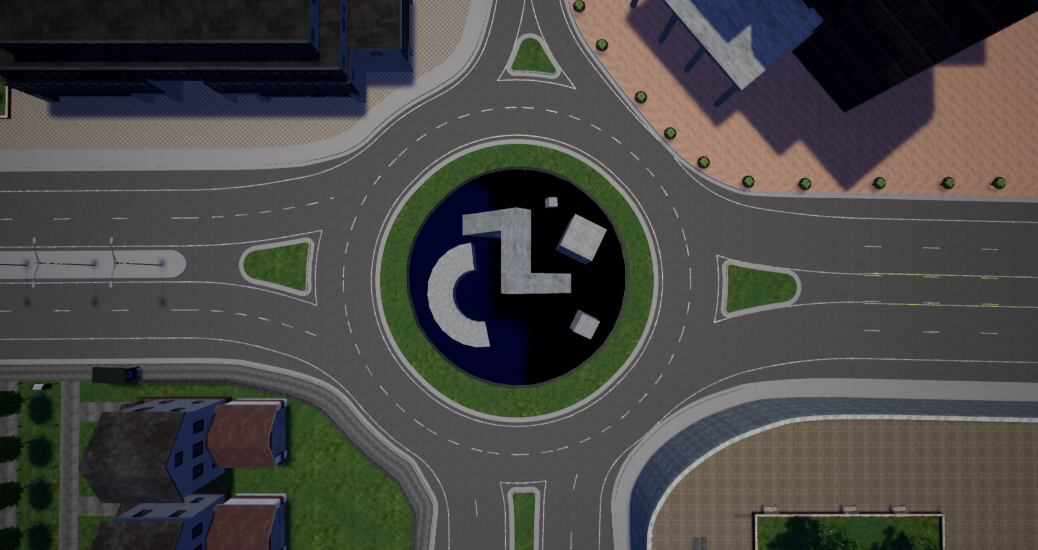
\includegraphics[width=1\linewidth]{images/bundaran}
	\caption{Bundaran Simpang Empat}
	\label{fig:bundaran_town03}
\end{figure}

\subsubsection{Bundaran Tanpa Simpang}
Digunakan bundaran tanpa simpang seperti pada Gambar  \ref{fig:bundaran_tanpa_simpang}. Pada lingkungan ini, agent akan \textit{spawn }dari sebuah titik \textit{spawn} awal bundaran.
\begin{figure}[H] 
	\centering
	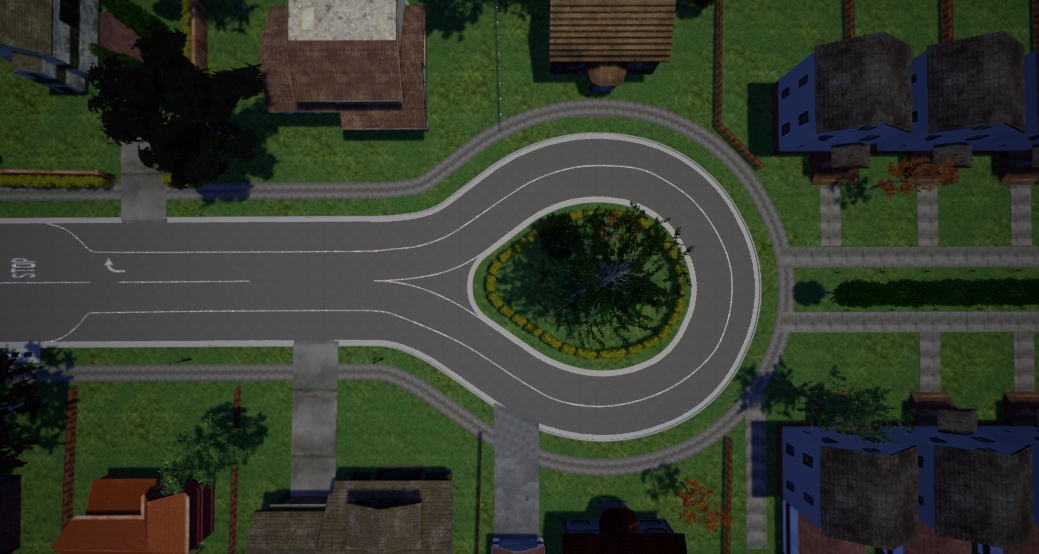
\includegraphics[width=1\linewidth]{images/bundaran_tanpa_simpang}
	\caption{Bundaran Tanpa Simpang}
	\label{fig:bundaran_tanpa_simpang}
\end{figure}

\subsection{Sensor}
\label{sec:sensor}
Sensor menggunakan sensor kamera yang diletakkan secara fisik di bagian depan bawah dari agen. Sensor kamera yang digunakan adalah sensor kamera segmentasi. Sensor kamera segmentasi adalah sensor kamera yang memisahkan object-object di simulator menjadi berbagai warna unik yang solid. Citra yang dihasilkan dari sensor kamera segmentasi pada Gambar \ref{fig:segmentasi} adalah citra lanjutan yang telah di proses dari citra RGB pada gambar \ref{fig:citra_rgb}


\subsection{Akuisisi Data}
\label{sec:akuisisi_data}
Data citra diambil dari sensor dengan ukuran 480x270. Citra yang digunakan adalah citra segmentasi yang telah disediakan oleh sensor kamera segmentasi dari CARLA Simulator. Terlihat pada Gambar \ref{fig:citra_rgb} merupakan citra awal. Kemudian dilakukan segmentasi pada citra tersebut sehingga setiap obyek dipresentasikan dengan warna solid seperti pada Gambar \ref{fig:segmentasi}

\begin{figure}[H] 
	\centering
	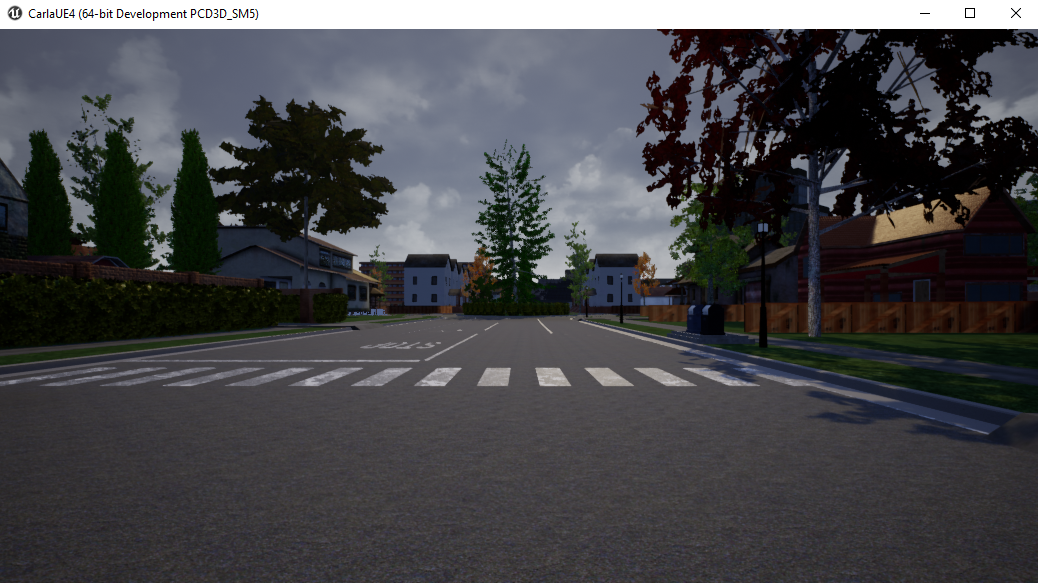
\includegraphics[width=1\linewidth]{images/rgb}
	\caption{Citra RGB}
	\label{fig:citra_rgb}
\end{figure}
\begin{figure}[H] 
	\centering
	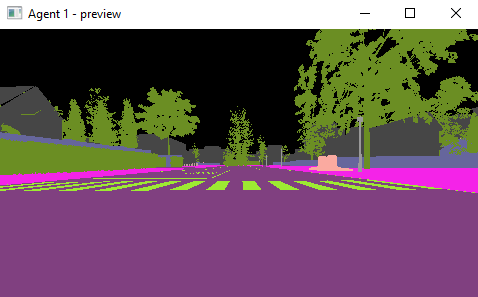
\includegraphics[width=1\linewidth]{images/segmentasi}
	\caption{Citra Segmentasi}
	\label{fig:segmentasi}
\end{figure}
Ada dua jenis citra yang digunakan dalam penelitian ini, yaitu citra segmentasi grayscale dan citra segmentasi lanjutan.

Citra segmentasi grayscale merupakan citra segmentasi yang kemudian diberi filter grayscale agar dapat meminimalkan data yang dianalisa namun tetap mempertahankan fitur yang ada.

\begin{figure}[H] 
	\centering
	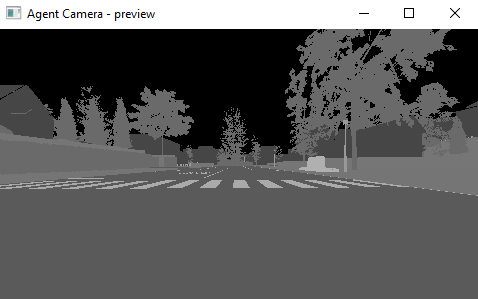
\includegraphics[width=1\linewidth]{images/grayscale}
	\caption{Citra Segmentasi Grayscale}
	\label{fig:grayscale}
\end{figure}

Citra segmentasi lanjutan merupakan citra segmentasi, yang kemudian di segmentasi kembali menjadi dua jenis obyek, yaitu \textit{drivable }dan \textit{non-drivable}. Obyek \textit{drivable} dipresentasikan dengan warna putih dan obyek \textit{non-drivable} dipresentasikan dengan warna hitam.

\begin{figure}[H] 
	\centering
	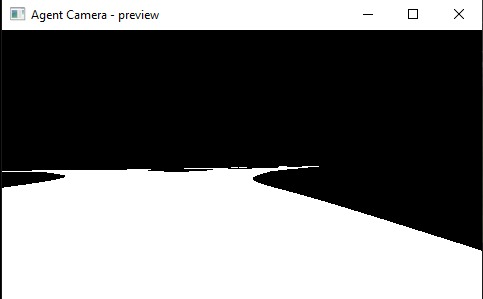
\includegraphics[width=1\linewidth]{images/segmentasi_hitam_putih}
	\caption{Citra Segmentasi Lanjutan}
	\label{fig:segmentasi_hitam_putih}
\end{figure}

Citra segmentasi grayscale dan citra segmentasi lanjutan akan menjadi hasil akhir akuisi citra yang kemudian akan diberikan ke algoritma DQN untuk melakukan \textit{training} model dan/atau \textit{inference} model.

\subsection{\textit{Action}}
\label{sec:action}
Ada 3 \textit{action} yang bisa dilakukan oleh \textit{agent}. Diantaranya:

\begin{enumerate}[nolistsep]
	\item \verb=forward=
	
	\textit{Agent} \textit{throttle} dengan nilai 1 dan \textit{steer} dengan nilai 0. Dengan demikian agent akan melakukan gerakan manuver maju.
	
	\item \verb=forward_left=
	
	Agen \textit{throttle} dengan nilai 1 dan \textit{steer} dengan nilai -1. Dengan demikian agent akan melakukan gerakan manuver maju ke depan kiri.
	
	\item \verb=forward_right=
	
	Agen \textit{throttle} dengan nilai 1 dan \textit{steer} dengan nilai 1. Dengan demikian agent akan melakukan gerakan manuver maju ke depan kanan.
	
\end{enumerate}

\subsection{\textit{Reward Function}}
\label{sec:sistem_reward}

Fungsi reward dirancang agar mobil otonom mampu bergerak sepanjang lintasan dengan cepat dan aman.

\subsubsection{Bundaran Simpang Empat}Ada dua buah reward yang ditetapkan dimana masing-masing reward memperhatikan referensi \textit{target lane}. Target lane adalah garis imajiner yang menjadi target gerakan mobil otonom. Terlihat pada Gambar \ref{fig:target_lane_line}, \textit{target lane} digambarkan dengan titik-titik merah di sekitar bundaran.

\begin{figure}[H] 
	\centering
	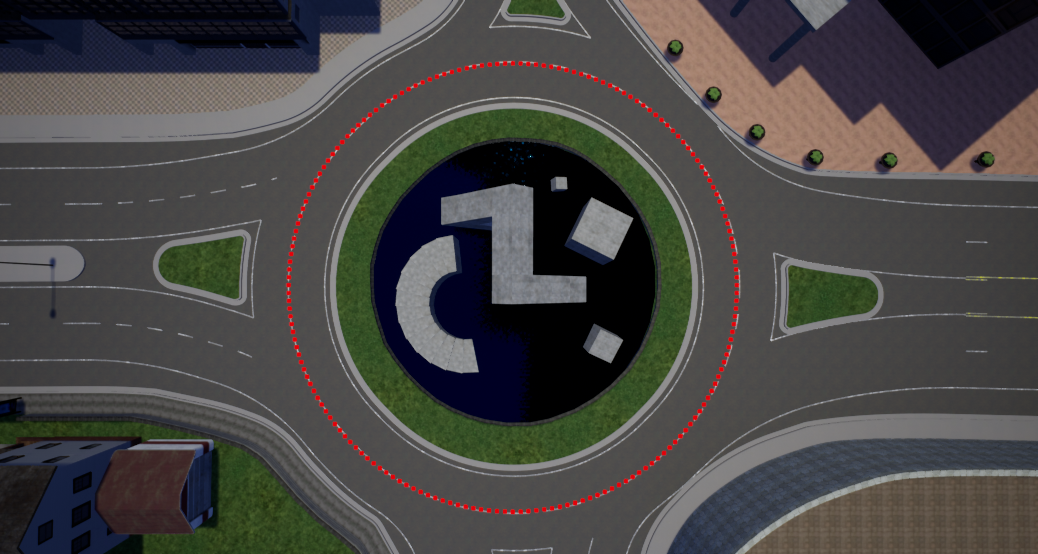
\includegraphics[width=1\linewidth]{images/target_lane_line}
	\caption{\textit{Target lane}}
	\label{fig:target_lane_line}
\end{figure}

\begin{enumerate}
\item \textit{Reward} 1: Deviasi sudut dari \textit{target lane}
Reward yang digunakan pada Reward 1 adalah 1/alpha. Alpha adalah sudut agent yang menyimpang dari \textit{target lane}. Teknis alpha dijelaskan pada Gambar \ref{fig:reward_anglediff_sketch}. 

\begin{figure}[H] 
	\centering
	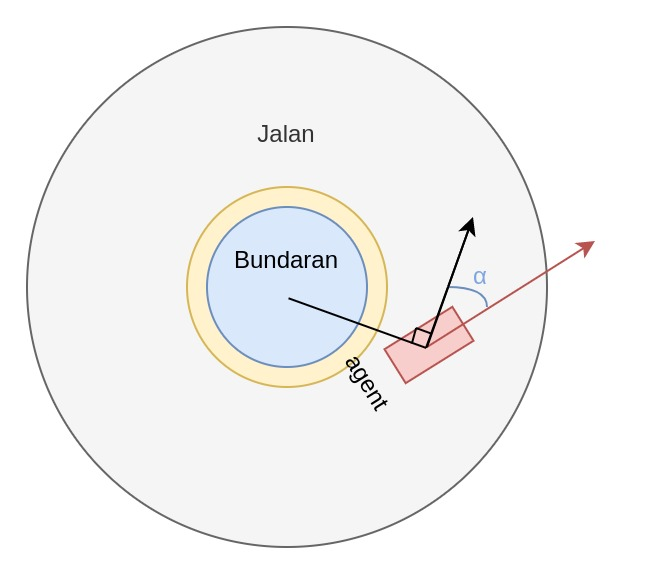
\includegraphics[width=1\linewidth]{images/reward_anglediff_sketch}
	\caption{Reward 1}
	\label{fig:reward_anglediff_sketch}
\end{figure}

Garis hitam merupakan vektor tegak lurus antara titik pusat bundaran ke titik pusat agen. Lalu garis merah adalah vektor arah mobil. Dari kedua nilai tersebut, didapat alpha yang merupakan sudut dari kedua vektor tersebut. Kemudian nilai reward didefinisikan dengan 1/alpha. Nilai tertinggi reward dibatasi menjadi 1. Hal ini dilakukan agar fluktuasi reward yang diberikan ke agent tidak terlalu tinggi untuk perubahan nilai yang kecil.


\item{\textit{Reward} 2: Deviasi jarak dari \textit{target lane}}
Reward yang digunakan pada reward 2 adalah \verb=1/deviasi_jarak*10=. Deviasi jarak adalah jarak terkecil agen terhadap \textit{target lane} dalam meter.

\begin{figure}[H] 
	\centering
	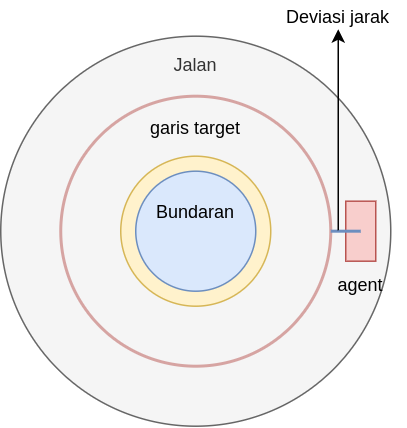
\includegraphics[width=.85\linewidth]{images/reward_deviasi_jarak}
	\caption{Reward 2}
	\label{fig:reward_deviasi_jarak}
\end{figure}
Nilai tertinggi reward dibatasi menjadi 1. Hal ini dilakukan agar fluktuasi reward yang diberikan ke agent juga tidak terlalu tinggi untuk perubahan nilai yang kecil, seperti pada Reward 1.


Selain reward yang bernilai positif, diperlukan juga reward yang bernilai negatif untuk mengurangi peluang agent melakukan hal yang sebaiknya tidak dilakukan. Ada dua buah reward bernilai negatif yang diberikan.

\item{\textit{Reward} 3: Sentuhan dengan obyek lain}
Reward senilai -1 akan diberikan pada \textit{agent} jika agent menyentuh obyek lain selain jalan raya, tanah, dan trotoar.

\item{\textit{Reward} 4: Deviasi jarak terlalu besar}
Reward senilai -0.5 akan diberikan pada \textit{agent} jika jarak antara \textit{agent} dan bundaran lebih besar dari 30 meter. Jarak 30 meter dari bundaran dapat dilihat di Gambar \ref{fig:punishment_lane_line}

\begin{figure}[H] 
	\centering
	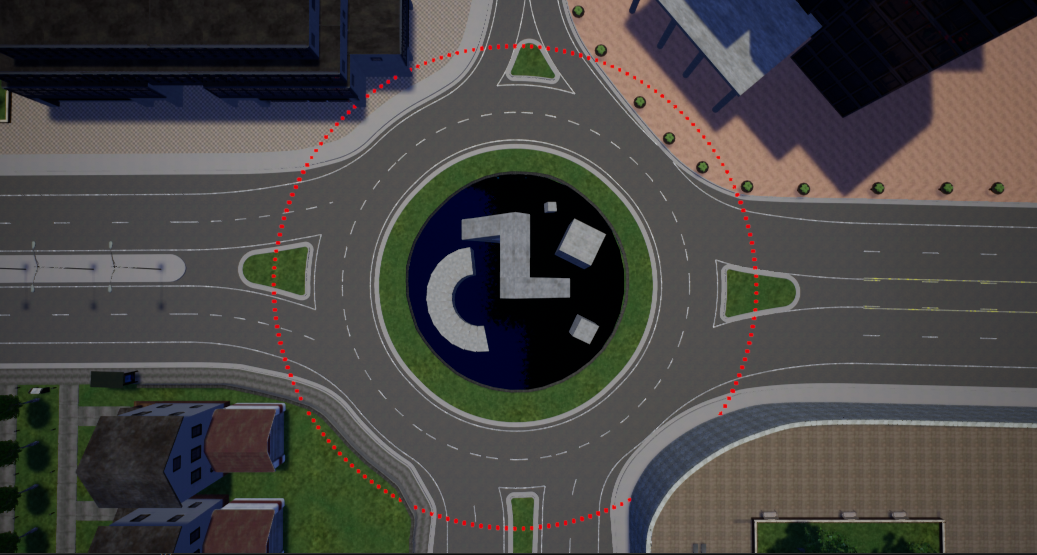
\includegraphics[width=1\linewidth]{images/punishment_lane_line}
	\caption{Batasan jarak}
	\label{fig:punishment_lane_line}
\end{figure}

\item{\textit{Reward }Total}
Total nilai reward didefinisikan dengan Reward 1 + Reward 2 + Reward 3 + Reward 4.

\end{enumerate}


\subsubsection{Bundaran Tanpa Simpang}
Pada bundaran tanpa simpang, fungsi reward yang diberikan berbeda. Pada kasus ini disediakan titik-titik jalur sebagai \textit{waypoint} yang harus diikuti oleh \textit{agent}.

\begin{figure}[H] 
	\centering
	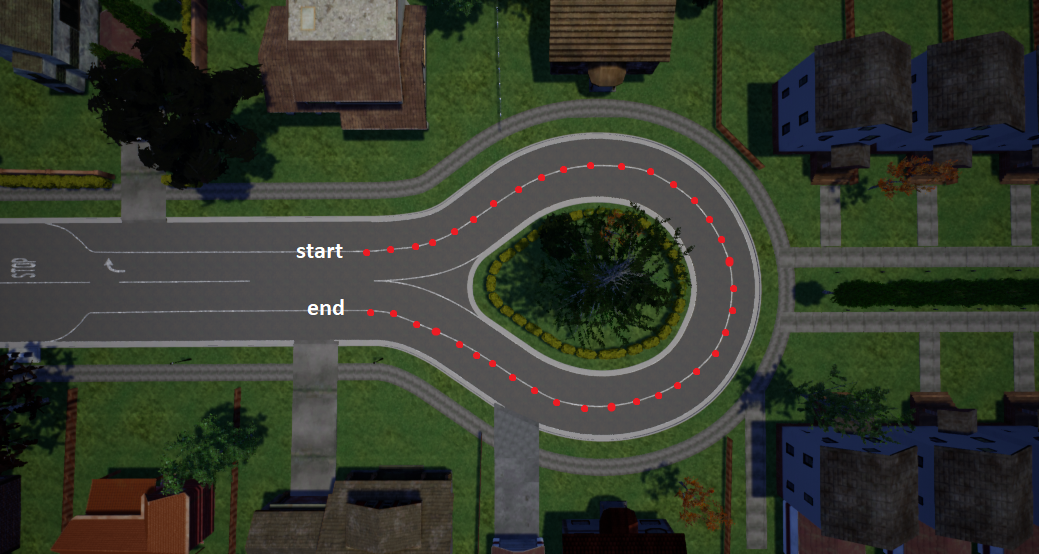
\includegraphics[width=1\linewidth]{images/waypoint}
	\caption{\textit{Waypoint}}
	\label{fig:waypoint}
\end{figure}

\textit{Waypoint} merupakan titik-titik pada map sebagai target tujuan jalannya \textit{agent}. Terlihat pada Gambar \ref{fig:waypoint}, titik-titik merah merupakan ilustrasi dari waypoint. Waypoint berjumlah 100 titik dimana setiap titiknya berjarak satu meter.

Reward didefinisikan dengan 1/alpha. Alpha merupakan deviasi sudut arah \textit{agent }terhadap arah titik \textit{waypoint} terdekat dari \textit{agent} + 5.

\begin{figure}[H] 
	\centering
	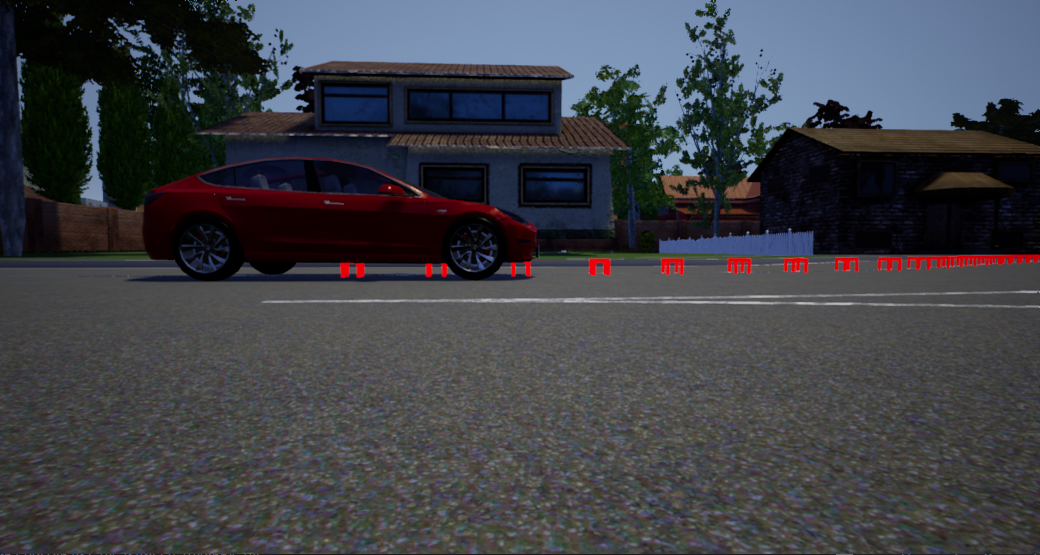
\includegraphics[width=1\linewidth]{images/waypoint_fromside}
	\caption{\textit{Waypoint }dari Sisi \textit{Agent}}
	\label{fig:waypoint_fromside}
\end{figure}

Gambar \ref{fig:waypoint_fromside} menunjukkan bahwa \textit{waypoint} terdekat + 5 dari \textit{agent} berjarak enam meter dari pusat koordinat \textit{agent}.

\begin{figure}[H] 
	\centering
	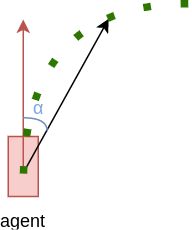
\includegraphics[width=.5\linewidth]{images/reward_alpha}
	\caption{Reward Alpha}
	\label{fig:reward_alpha}
\end{figure}

Ilustrasi fungsi reward dapat dilihat pada Gambar \ref{fig:reward_alpha}, dimana titik-titik hijau adalah \textit{waypoints}, garis merah adalah arah dari \textit{agent}, garis hitam adalah arah dari \textit{agent} ke \textit{waypoint}+5 dari \textit{agent}, serta alpha adalah perbedaan sudut dari kedua nilai sudut tersebut. Nilai tertinggi reward dibatasi menjadi 1. Hal ini dilakukan agar fluktuasi reward yang diberikan ke agent juga tidak terlalu tinggi untuk perubahan nilai yang kecil, seperti pada Reward 1 dan Reward 2 pada bundaran simpang empat.


\subsubsection{End Episode}
\label{sec:end_episode}
Waktu maksimal yang diberikan pada agent untuk melakukan proses learning setiap episodenya adalah 10 detik.

Episode akan berakhir jika waktu maksimal episode berakhir atau agent menyentuh object lain selain jalan raya, tanah, dan trotoar.

\subsection{Parameter DQN}
\label{sec:parameter_dqn}
Penentuan nilai hyperparameter yang tepat merupakan salah satu langkah yang penting dilakukan untuk mendapatkan model pembelajaran mesin yang baik. Dalam machine learning, hyperparameter adalah parameter yang digunakan untuk mengatur jalannya proses pembelajaran mesin. Berbeda dengan parameter model yang nilainya mengalami perubahan seiring berjalannya pembelajaran mesin, hyperparameter perlu didefinisikan di awal dan umumnya bernilai tetap sepanjang proses pembelajaran. Dalam penelitian ini, hyperparameter dari algoritma DQN didefinisikan sebagai berikut:

\subsubsection{Model}
\label{sec:model}
\begin{table}[H]
	\resizebox{\columnwidth}{!}{%
		\begin{tabular}{|l|l|l|}
			\hline
			\textbf{Hyperparameter}   & \textbf{Nilai} & \textbf{Deskripsi}                                                                                                                            \\ \hline
			MINIBATCH\_SIZE           & 16             & \begin{tabular}[c]{@{}l@{}}Jumlah sampel pembelajaran yang\\ diproses oleh perhitungan SGD\\ (stochastic gradient) algoritma DQN\end{tabular} \\ \hline
			PREDICTION\_BATCH\_SIZE   & 1              & \begin{tabular}[c]{@{}l@{}}Jumlah sampel yang di prediksi\\ di saat yang bersamaan\end{tabular}                                               \\ \hline
			TRAINING\_BATCH\_SIZE     & 8              & \begin{tabular}[c]{@{}l@{}}Jumlah sampel yang di fit di saat\\ yang bersamaan (lebih besar lebih\\ cepat)\end{tabular}                        \\ \hline
			TRAINER\_MEMORY\_FRACTION & 0.6            &                                                                                                                                               \\ \hline
		\end{tabular}%
	}
	\caption{Hyperparameter model.}
	\label{tb:hyperparameter_model}
\end{table}

\iffalse
\begin{verbatim}
	MINIBATCH_SIZE = 16
	PREDICTION_BATCH_SIZE = 1
	TRAINING_BATCH_SIZE = MINIBATCH_SIZE // 2
	UPDATE_TARGET_EVERY = 100
	TRAINER_MEMORY_FRACTION = 0.6
	SAVE_CHECKPOINT_EVERY = 50
\end{verbatim}
\fi

\subsubsection{DQN}
\label{sec:dqn}

\begin{table}[H]
	\resizebox{\columnwidth}{!}{%
		\begin{tabular}{|l|l|l|}
			\hline
			\textbf{Hyperparameter}   & \textbf{Nilai} & \textbf{Deskripsi}                                                                                                                            \\ \hline
			DISCOUNT                  & 0.99           & \begin{tabular}[c]{@{}l@{}}Nilai faktor discount dalam\\ perhitungan reward algoritma DQN\end{tabular}                                        \\ \hline
			REPLAY\_MEMORY\_SIZE      & 20\_000        & \begin{tabular}[c]{@{}l@{}}Berapa banyak step terakhir yang\\ disimpan untuk training model\end{tabular}                                      \\ \hline
			MIN\_REPLAY\_MEMORY\_SIZE & 5\_000         & \begin{tabular}[c]{@{}l@{}}Jumlah step minimum dalam\\ memori untuk memulai training\end{tabular}                                             \\ \hline
			OPTIMIZER\_LEARNING\_RATE & 0.001          & \begin{tabular}[c]{@{}l@{}}Laju pembelajaran yang digunakan\\ pada optimizer\end{tabular}                                                     \\ \hline
			OPTIMIZER\_DECAY          & 0.0            & \begin{tabular}[c]{@{}l@{}}Pengurangan laju pembelajaran\\ pada optimizer setiap episodenya\end{tabular}                                      \\ \hline
		\end{tabular}%
	}
	\caption{Hyperparameter DQN.}
	\label{tb:hyperparameter_dqn}
\end{table}

\iffalse
\begin{verbatim}
	DISCOUNT = 0.99
	REPLAY_MEMORY_SIZE = 20_000
	MIN_REPLAY_MEMORY_SIZE = 5_000
\end{verbatim}
\fi

\subsubsection{Epsilon}

\begin{table}[H]
	\resizebox{\columnwidth}{!}{%
		\begin{tabular}{|l|l|l|}
			\hline
			\textbf{Hyperparameter}   & \textbf{Nilai} & \textbf{Deskripsi}                                                                                                                            \\ \hline
			
			START\_EPSILON            & 1              & \begin{tabular}[c]{@{}l@{}}Nilai epsilon saat pertamakali\\ mulai training\end{tabular}                                                       \\ \hline
			EPSILON\_DECAY            & 0.9995         & \begin{tabular}[c]{@{}l@{}}Penurunan nilai epsilon di setiap\\ episodenya\end{tabular}                                                        \\ \hline
			MIN\_EPSILON              & 0.1            & \begin{tabular}[c]{@{}l@{}}Epsilon terendah yang\\ diperbolehkan\end{tabular}                                                                 \\ \hline
		\end{tabular}%
	}
	\caption{Hyperparameter epsilon.}
	\label{tb:hyperparameter_epsilon}
\end{table}
Penentuan parameter epsilon ditentukan oleh kondisi berikut. Epsilon akan bernilai 1 saat pertamakali memulai learning atau pada saat episode 0. Setiap dimulainya episode baru, nilai epsilon akan dikali dengan nilai 0.9995 hingga pada akhirnya akan bernilai 0.1 setelah 4700 episode. Pengurangan nilai epsilon akan berhenti setelah sampai pada nilai 0.1.

Penentuan parameter \textit{epsilon-greedy} ini dilakukan agar agent mampu melakukan kegiatan eksplorasi dan eksploitasi dengan tepat. Sehingga hasil yang didapatkan akan baik dalam waktu cepat.
\label{sec:epsilon}

\iffalse
\begin{verbatim}
	START_EPSILON = 1
	EPSILON_DECAY = 0.9995
	MIN_EPSILON = 0.1
\end{verbatim}
\fi

\subsection{Arsitektur Model}
\label{sec:arsitektur_model}

Berikut adalah arsitektur yang digunakan:

\begin{table}[H]
	\begin{tabular}{lll}
		\textbf{Layer (type)}                      & \textbf{Output Shape}         & \textbf{Param \#} \\
		conv2d\_1\_input (InputLayer)     & (None, 270, 480, 1)  & 0        \\
		conv2d\_1 (Conv2D)                & (None, 270, 480, 64) & 640      \\
		activation\_1 (Activation)        & (None, 270, 480, 64) & 0        \\
		average\_pooling2d\_1 (AveragePoo & (None, 90, 160, 64)  & 0        \\
		conv2d\_2 (Conv2D)                & (None, 90, 160, 64)  & 36928    \\
		activation\_2 (Activation)        & (None, 90, 160, 64)  & 0        \\
		average\_pooling2d\_2 (AveragePoo & (None, 30, 54, 64)   & 0        \\
		conv2d\_3 (Conv2D)                & (None, 30, 54, 64)   & 36928    \\
		activation\_3 (Activation)        & (None, 30, 54, 64)   & 0        \\
		average\_pooling2d\_3 (AveragePoo & (None, 10, 18, 64)   & 0        \\
		flatten\_1 (Flatten)              & (None, 11520)        & 0        \\
		kmh\_input (InputLayer)           & (None, 1)            & 0        \\
		concatenate\_1 (Concatenate)      & (None, 11521)        & 0        \\
		dense\_1 (Dense)                  & (None, 256)          & 2949632  \\
		dense\_2 (Dense)                  & (None, 3)            & 771     
	\end{tabular}
	\caption{Arsitektur model.}
	\label{tb:arsitektur_model}
\end{table}

Diberikan konvolusi kepada citra image sebanyak 3 kali. Setiap konvolusi dilakukan dengan average pooling. Proses selanjutnya setelah konvolusi adalah menambahkan data kecepatan agent. Kemudian pada akhir dari proses akan didapatkan output action berjumlah 3.

\subsection{Training}
\label{sec:training}

\begin{figure}[H] 
	\centering
	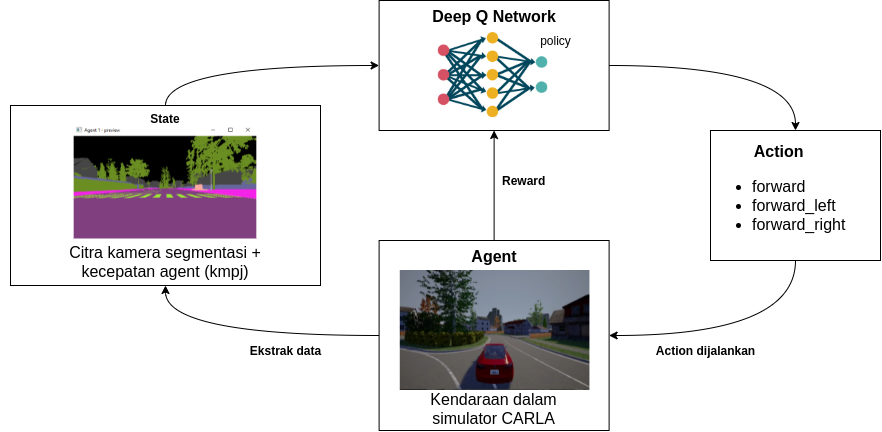
\includegraphics[width=1\linewidth]{images/metodologi}
	\caption{Diagram Blok Metodologi}
	\label{fig:blockdiagram}
\end{figure}

Proses training dilakukan setelah seluruh konfigurasi selesai dilakukan. Metodologi training dari penelitian ini terdapat pada Gambar \ref{fig:blockdiagram}. \textit{Agent} yang berada pada simulasi melakukan suatu \textit{action} yang menyebabkan berubahnya \textit{state}. \textit{State} yang berupa citra segmentasi dan kecepatan agent (kmpj) serta \textit{reward }dari \textit{agent} kemudian dikirimkan ke DQN untuk dilakukan training. Hasil dari training berupa \textit{policy },  akan menentukan\textit{action} yang kemudian akan dilaksanakan oleh \textit{agent}. Kemudian proses tersebut akan terulang kembali menjadi sebuah siklus yang tak henti.

	
	
	
	\section{Testing and Result}
	\subsection{Training DQN}
	\label{sec:training_dqn}
	Training algoritma DQN dilakukan dengan menggunakan hardware berikut:
	\begin{table}[H]
		\begin{tabular}{ll}
			\textbf{CPU}  & Intel Core i5              \\
			\textbf{GPU}  & Nvidia GTX 1060 - 6GB VRAM \\
			\textbf{RAM}  & 8GB                        \\
			\textbf{Disk} & 256GB SSD M.2              \\
			\textbf{OS}   & Windows 10                
		\end{tabular}
		\caption{Hardware yang digunakan untuk learning.}
		\label{tb:hardwaresetup}
	\end{table}
	
	Learning dilakukan dengan mesin lokal menggunakan GPU. Lingkungan software machine learning yang digunakan pada learning berupa:
	
	\begin{table}[H]
		\begin{tabular}{ll}
			\textbf{Software}  & \textbf{Version}              \\
			tensorflow-gpu  & 1.13.1	\\
			keras  & 2.2.5					\\
			h5py & 3.1              \\
			python & 3.7.9              \\
		\end{tabular}
		\caption{Lingkungan software yang digunakan untuk learning.}
		\label{tb:softwaresetup}
	\end{table}
	
	
	Hasil dari proses training tersebut adalah model jaringan DQN yang merepresentasikan sistem perencanaan gerakan mobil otonom. Model tersebut disimpan dalam sebuah file berformat .model yang
	selanjutnya dapat divisualisasikan dengan tensorboard untuk melihat hasil training algoritma DQN. 
	
	\subsection{Training DQN pada Bundaran Simpang Empat dengan Segmentasi Grayscale}
	\label{sec:training_dqn_bundaran_simpangempat_segmentasi_grayscale}
	
	Training algoritma DQN pada bundaran simpang empat dengan segmentasi grayscale berlangsung selama 20 jam. Berikut adalah hasil visualisasi training algoritma DQN:
	
	\begin{figure}[H] 
		\centering
		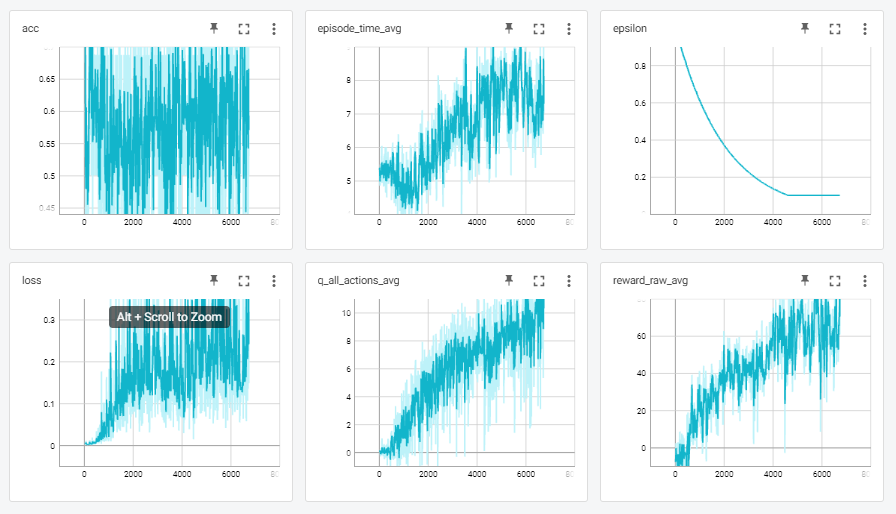
\includegraphics[width=1\linewidth]{images/tensorboard_bundaran_simpangempat_segmentasi_grayscale}
		\caption{Tensorboard pada Bundaran Simpang Empat dengan Segmentasi Grayscale}
		\label{fig:tensorboard_bundaran_simpangempat_segmentasi_grayscale}
	\end{figure}
	
	Dari hasil visualisasi training DQN pada Gambar \ref{fig:tensorboard_bundaran_simpangempat_segmentasi_grayscale}, dapat dilihat bahwa proses training algoritma DQN telah berjalan dengan baik. Hal itu dapat dilihat dari nilai akurasi, episode time, dan reward berkendara mobil otonom yang mengalami tren kenaikan seiring dengan berjalannya proses training.
	
	\subsection{Training DQN pada Bundaran Simpang Empat dengan Segmentasi Lanjutan}
	\label{sec:training_dqn_bundaran_simpangempat_segmentasi_hitam_putih}
	
	Training algoritma DQN pada bundaran simpang empat dengan segmentasi lanjutan berlangsung selama 13 jam, 30 menit, dan 48 detik. Berikut adalah hasil visualisasi training algoritma DQN:
	
	\begin{figure}[H] 
		\centering
		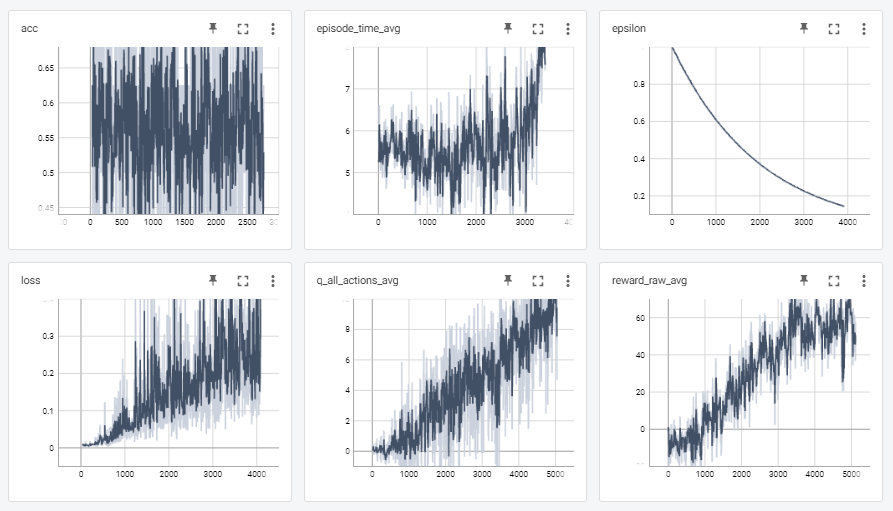
\includegraphics[width=1\linewidth]{images/tensorboard_bunderan_segmented}
		\caption{Tensorboard pada Bundaran Simpang Empat dengan Segmentasi Lanjutan}
		\label{fig:tensorboard_bundaran_simpangempat_segmentasi_lanjutan}
	\end{figure}
	
	Dari hasil visualisasi training DQN pada Gambar \ref{fig:tensorboard_bundaran_tanpasimpang_segmentasi_lanjutan}, dapat dilihat bahwa proses training algoritma DQN telah berjalan dengan baik. Hal itu dapat dilihat dari nilai akurasi, episode time, dan reward berkendara mobil otonom yang mengalami tren kenaikan seiring dengan berjalannya proses training.
	
	
	\subsection{Training DQN pada Bundaran Tanpa Simpang dengan Segmentasi Lanjutan}
	\label{sec:training_dqn_bundaran_nosimpang_segmentasi_hitam_putih}
	
	Training algoritma DQN pada bundaran tanpa simpang dengan segmentasi lanjutan berlangsung selama 26 jam dan 25 detik. Berikut adalah hasil visualisasi training algoritma DQN:
	
	\begin{figure}[H] 
		\centering
		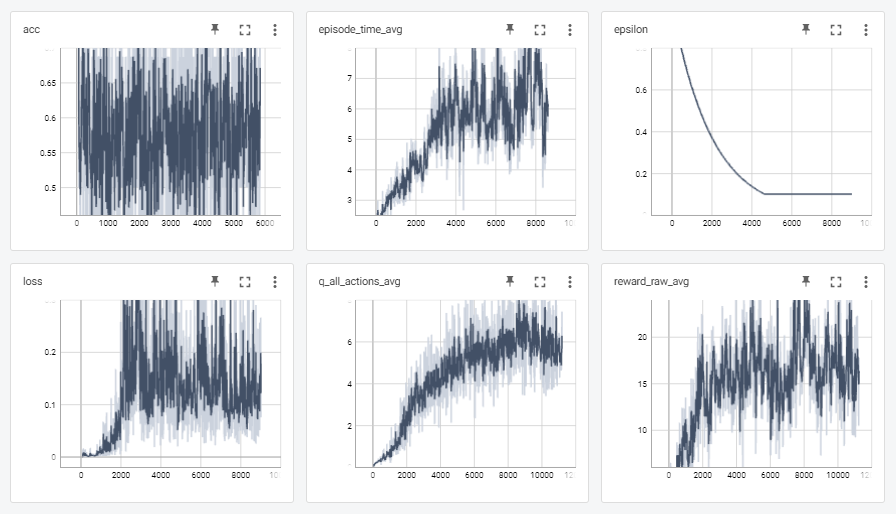
\includegraphics[width=1\linewidth]{images/tensorboard_itemputih_nosimpang}
		\caption{Tensorboard pada Bundaran Tanpa Simpang dengan Segmentasi Lanjutan}
		\label{fig:tensorboard_bundaran_tanpasimpang_segmentasi_lanjutan}
	\end{figure}
	
	Dari hasil visualisasi training DQN pada Gambar \ref{fig:tensorboard_bundaran_tanpasimpang_segmentasi_lanjutan}, dapat dilihat bahwa proses training algoritma DQN telah berjalan dengan baik. Hal itu dapat dilihat dari nilai akurasi, episode time, dan reward berkendara mobil otonom yang mengalami tren kenaikan seiring dengan berjalannya proses training.
	
	
	\iffalse
	Training algoritma DQN dengan
	berlangsung selama 81 jam, 12 menit, dan 38 detik. Berikut adalah hasil visualisasi training algoritma DQN:
	
	\begin{figure}[H] 
		\centering
		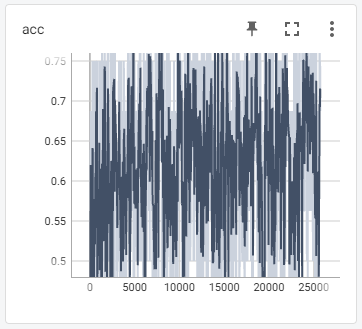
\includegraphics[width=.7\linewidth]{images/acc}
		\caption{Nilai akurasi}
		\label{fig:acc}
	\end{figure}
	\begin{figure}[H] 
		\centering
		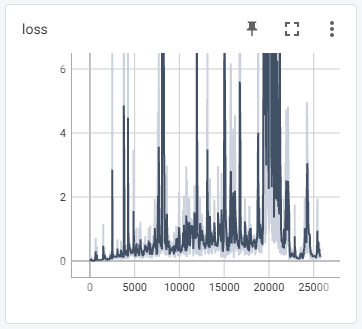
\includegraphics[width=.7\linewidth]{images/loss}
		\caption{Nilai loss}
		\label{fig:loss}
	\end{figure}
	\begin{figure}[H] 
		\centering
		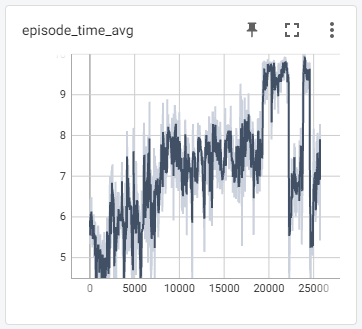
\includegraphics[width=.7\linewidth]{images/episode_time_avg}
		\caption{Rerata waktu episode}
		\label{fig:episode_time_avg}
	\end{figure}
	\begin{figure}[H] 
		\centering
		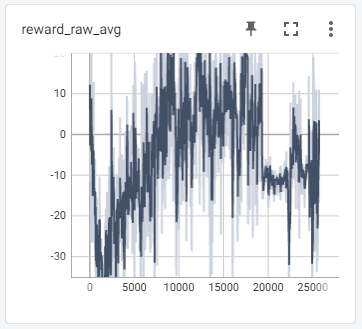
\includegraphics[width=.7\linewidth]{images/reward_raw_avg}
		\caption{Rerata nilai reward \textit{raw}}
		\label{fig:reward_raw_avg}
	\end{figure}
	\begin{figure}[H] 
		\centering
		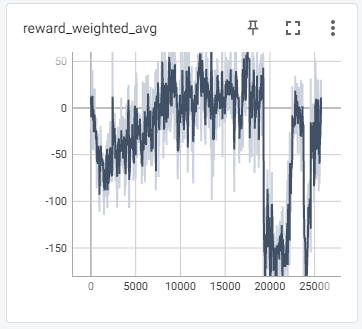
\includegraphics[width=.7\linewidth]{images/reward_weighted_avg}
		\caption{Rerata nilai reward \textit{weighted}}
		\label{fig:reward_weighted_avg}
	\end{figure}
	\begin{figure}[H] 
		\centering
		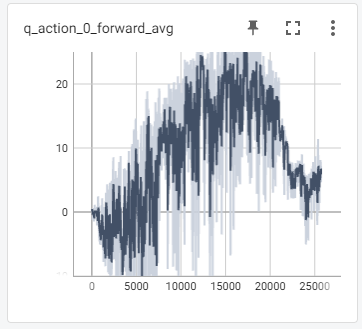
\includegraphics[width=.7\linewidth]{images/q_action_0_forward_avg}
		\caption{Nilai rerata q dari action forward}
		\label{fig:q_action_0_forward_avg}
	\end{figure}
	\begin{figure}[H] 
		\centering
		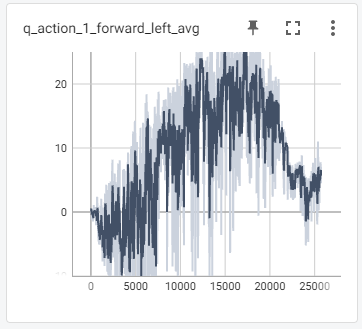
\includegraphics[width=.7\linewidth]{images/q_action_1_forward_left_avg}
		\caption{Nilai rerata q dari action forward left}
		\label{fig:q_action_1_forward_left_avg}
	\end{figure}
	\begin{figure}[H] 
		\centering
		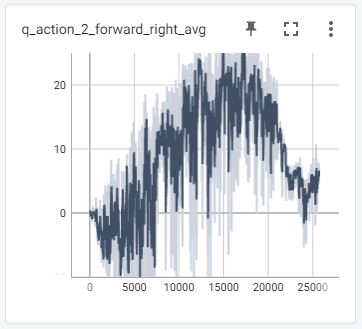
\includegraphics[width=.7\linewidth]{images/q_action_2_forward_right_avg}
		\caption{Nilai rerata q dari action forward right}
		\label{fig:q_action_2_forward_right_avg}
	\end{figure}
	\begin{figure}[H] 
		\centering
		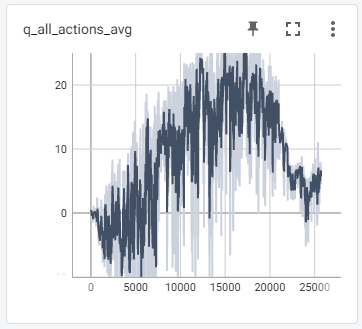
\includegraphics[width=.7\linewidth]{images/q_all_actions_avg}
		\caption{Nilai rerata q dari seluruh action}
		\label{fig:q_all_actions_avg}
	\end{figure}
	
	Dari hasil visualisasi training DQN diatas, dapat dilihat bahwa proses training algoritma DQN telah berjalan dengan baik. Hal itu dapat dilihat dari nilai akurasi, \textit{episode time}, dan \textit{reward} berkendara mobil otonom yang mengalami tren kenaikan seiring dengan berjalannya proses training.
	
	\fi
	
	\section{Pengujian Model DQN}
	\label{sec:pengujian_model_dqn}
	
	Pada bagian ini, akan dilakukan pengujian model hasil dari proses training DQN. Pengujian dilakukan saat lingkungan berkendara dalam kondisi normal.
	
	\subsection{Pengujian Model DQN pada Bundaran Simpang Empat dengan Segmentasi Grayscale}
	\label{sec:pengujian_dqn_bundaran_simpangempat_segmentasi_grayscale}
	
	% Please add the following required packages to your document preamble:
	% \usepackage{graphicx}
	\begin{table}[H]
		\resizebox{\columnwidth}{!}{%
			\begin{tabular}{|l|l|l|l|l|}
				\hline
				episode\_length & avg\_speed & avg\_angle\_diff & avg\_dist\_diff & avg\_reward \\ \hline
				9.005           & 34.983     & 20.001           & 5.812           & 0.166       \\ \hline
				4.772           & 28.927     & 12.14            & 0.91            & 0.448       \\ \hline
				8.524           & 33.052     & 10.65            & 1.993           & 0.398       \\ \hline
				12.678          & 35.053     & 15.259           & 3.264           & 0.222       \\ \hline
				13.621          & 37.03      & 32.642           & 12.394          & 0.122       \\ \hline
				4.851           & 30.102     & 10.241           & 1.253           & 0.471       \\ \hline
				6.555           & 20.433     & 21.37            & 2.775           & 0.318       \\ \hline
				8.694           & 31.494     & 14.927           & 3.381           & 0.235       \\ \hline
				20.184          & 34.142     & 58.799           & 45.228          & -0.23       \\ \hline
				10.026          & 28.305     & 12.737           & 2.411           & 0.332       \\ \hline
				5.147           & 29.648     & 17.682           & 1.707           & 0.289       \\ \hline
				8.521           & 32.238     & 13.255           & 2.253           & 0.289       \\ \hline
				7.99            & 32.617     & 13.939           & 2.661           & 0.342       \\ \hline
				5.206           & 30.142     & 13.541           & 1.077           & 0.409       \\ \hline
				6.072           & 23.77      & 36.641           & 3.617           & 0.17        \\ \hline
				5.426           & 31.166     & 12.926           & 0.925           & 0.418       \\ \hline
				5.176           & 27.477     & 12.276           & 1.194           & 0.457       \\ \hline
				8.085           & 33.884     & 11.883           & 1.224           & 0.343       \\ \hline
				10.048          & 27.918     & 15.146           & 3.086           & 0.306       \\ \hline
				7.443           & 33.063     & 12.29            & 2.298           & 0.383       \\ \hline
				29.772          & 38.947     & 65.564           & 58.657          & -0.255      \\ \hline
				6.617           & 30.019     & 20.405           & 1.658           & 0.425       \\ \hline
				4.931           & 27.362     & 12.078           & 1.821           & 0.361       \\ \hline
				14.428          & 29.973     & 18.9             & 3.066           & 0.272       \\ \hline
				5.445           & 30.364     & 10.48            & 0.951           & 0.523       \\ \hline
				8.794           & 31.964     & 15.54            & 2.635           & 0.294       \\ \hline
				8.568           & 33.002     & 13.103           & 1.95            & 0.409       \\ \hline
				20.471          & 24.614     & 64.263           & 15.817          & -0.076      \\ \hline
				5.276           & 31.54      & 14.182           & 1.594           & 0.349       \\ \hline
				7.645           & 29.516     & 39.559           & 1.573           & 0.349       \\ \hline
			\end{tabular}%
		}
		\caption{30 Sampel Hasil Model DQN pada Bundaran Simpang Empat dengan Segmentasi Grayscale.}
		\label{tb:hasilpengujian_bunderan_grayscale}
	\end{table}
	
	Dari hasil pengambilan sampel tersebut didapatkan kesimpulan seperti pada tabel \ref{tb:kesimpulan_bunderan_grayscale}.
	
	% Please add the following required packages to your document preamble:
	% \usepackage{graphicx}
	\begin{table}[H]
		\resizebox{\columnwidth}{!}{%
			\begin{tabular}{|l|l|l|l|l|}
				\hline
				avg\_episode\_length & avg\_speed & avg\_angle\_diff & avg\_dist\_diff & avg\_reward \\ \hline
				9.332                & 30.758     & 21.413           & 6.306           & 0.284       \\ \hline
			\end{tabular}%
		}
		\caption{Kesimpulan Hasil Model DQN pada Bundaran Simpang Empat dengan Segmentasi Grayscale.}
		\label{tb:kesimpulan_bunderan_grayscale}
	\end{table}
	
	
	
	\subsection{Pengujian Model DQN pada Bundaran Simpang Empat dengan Segmentasi Lanjutan}
	\label{sec:pengujian_dqn_bundaran_simpangempat_segmentasi_hitam_putih}
	
	\begin{table}[H]
		\resizebox{\columnwidth}{!}{%
			\begin{tabular}{|l|l|l|l|l|}
				\hline
				episode\_length & avg\_speed & avg\_angle\_diff & avg\_dist\_diff & avg\_reward \\ \hline
				7.431           & 38.229     & 10.205           & 2.0             & 0.34        \\ \hline
				8.094           & 30.83      & 24.743           & 1.187           & 0.392       \\ \hline
				8.418           & 30.337     & 20.039           & 2.106           & 0.257       \\ \hline
				21.587          & 37.044     & 14.712           & 2.588           & 0.28        \\ \hline
				7.019           & 35.495     & 11.015           & 0.849           & 0.465       \\ \hline
				19.252          & 35.029     & 20.848           & 3.259           & 0.267       \\ \hline
				18.607          & 29.382     & 58.62            & 6.881           & 0.071       \\ \hline
				6.529           & 36.715     & 10.4             & 1.301           & 0.348       \\ \hline
				14.337          & 36.066     & 16.105           & 0.99            & 0.421       \\ \hline
				17.025          & 34.249     & 45.883           & 4.252           & 0.15        \\ \hline
				9.511           & 41.363     & 12.647           & 1.503           & 0.32        \\ \hline
				36.864          & 34.917     & 68.418           & 8.128           & 0.069       \\ \hline
				9.973           & 38.902     & 13.901           & 1.56            & 0.304       \\ \hline
				7.34            & 35.594     & 13.333           & 1.547           & 0.45        \\ \hline
				14.864          & 31.482     & 59.456           & 3.588           & 0.112       \\ \hline
				9.987           & 41.68      & 12.595           & 1.952           & 0.297       \\ \hline
				9.767           & 39.018     & 15.001           & 1.341           & 0.373       \\ \hline
				7.011           & 36.749     & 10.62            & 1.488           & 0.321       \\ \hline
				17.4            & 26.631     & 79.254           & 13.336          & -0.07       \\ \hline
				12.798          & 40.187     & 15.749           & 1.645           & 0.285       \\ \hline
				17.809          & 31.448     & 46.125           & 2.951           & 0.268       \\ \hline
				11.504          & 36.149     & 21.827           & 1.347           & 0.355       \\ \hline
				6.395           & 37.127     & 9.601            & 0.895           & 0.418       \\ \hline
				23.591          & 30.945     & 60.991           & 4.07            & 0.153       \\ \hline
				6.957           & 37.284     & 8.505            & 0.959           & 0.438       \\ \hline
				9.431           & 40.093     & 11.436           & 1.98            & 0.311       \\ \hline
				35.604          & 27.912     & 80.507           & 11.311          & -0.171      \\ \hline
				9.089           & 42.26      & 10.891           & 1.286           & 0.395       \\ \hline
				7.032           & 36.387     & 11.418           & 1.278           & 0.418       \\ \hline
				8.578           & 34.796     & 15.489           & 1.456           & 0.316       \\ \hline
			\end{tabular}%
		}
		\caption{30 Sampel Hasil Model DQN pada Bundaran Simpang Empat dengan Segmentasi Lanjutan.}
		\label{tb:hasilpengujian_bunderan_segmented}
	\end{table}
	
	Dari hasil pengambilan sampel tersebut didapatkan kesimpulan seperti pada tabel \ref{tb:kesimpulan_bunderan_segmented}.
	
	
	% Please add the following required packages to your document preamble:
	% \usepackage{graphicx}
	\begin{table}[H]
		\resizebox{\columnwidth}{!}{%
			\begin{tabular}{|l|l|l|l|l|}
				\hline
				avg\_episode\_length & avg\_speed & avg\_angle\_diff & avg\_dist\_diff & avg\_reward \\ \hline
				13.326                & 35.476     & 27.011           & 2.967           & 0.278       \\ \hline
			\end{tabular}%
		}
		\caption{Kesimpulan Hasil Model DQN pada Bundaran Simpang Empat dengan Segmentasi Lanjutan.}
		\label{tb:kesimpulan_bunderan_segmented}
	\end{table}
	
	\subsection{Pengujian Model DQN pada Bundaran Tanpa Simpang dengan Segmentasi Lanjutan}
	\label{sec:pengujian_dqn_bundaran_nosimpang_segmentasi_hitam_putih}
	
	\begin{table}[H]
		\begin{tabular}{|l|l|l|l|}
			\hline
			episode\_length & avg\_speed  & avg\_alpha  & avg\_reward \\ \hline
			8.374           & 32.202 & 31.098 & 0.113  \\ \hline
			8.796           & 29.909 & 32.023 & 0.093  \\ \hline
			12.195          & 29.678 & 40.528 & 0.068  \\ \hline
			12.439          & 30.384 & 36.557 & 0.12   \\ \hline
			10.246          & 29.72  & 42.027 & 0.063  \\ \hline
			3.138           & 19.86  & 32.557 & 0.085  \\ \hline
			9.982           & 30.777 & 35.319 & 0.129  \\ \hline
			8.185           & 30.64  & 24.322 & 0.112  \\ \hline
			9.719           & 31.814 & 31.563 & 0.081  \\ \hline
			10.908          & 33.314 & 38.641 & 0.097  \\ \hline
			3.299           & 21.882 & 22.22  & 0.122  \\ \hline
			9.27            & 31.347 & 26.635 & 0.12   \\ \hline
			4.27            & 26.317 & 16.402 & 0.152  \\ \hline
			3.765           & 23.032 & 32.14  & 0.169  \\ \hline
			10.776          & 31.581 & 37.949 & 0.091  \\ \hline
			5.588           & 28.784 & 29.461 & 0.155  \\ \hline
			3.219           & 22.536 & 20.392 & 0.186  \\ \hline
			8.508           & 30.489 & 24.669 & 0.122  \\ \hline
			4.457           & 23.68  & 23.546 & 0.146  \\ \hline
			3.824           & 22.575 & 36.989 & 0.105  \\ \hline
			10.599          & 31.869 & 23.992 & 0.132  \\ \hline
			12.438          & 31.08  & 38.071 & 0.088  \\ \hline
			7.873           & 31.305 & 21.448 & 0.15   \\ \hline
			3.562           & 22.864 & 16.225 & 0.136  \\ \hline
			8.758           & 27.877 & 37.786 & 0.076  \\ \hline
			4.641           & 26.732 & 25.345 & 0.106  \\ \hline
			10.472          & 32.074 & 33.322 & 0.101  \\ \hline
			10.937          & 31.784 & 33.864 & 0.095  \\ \hline
			9.244           & 30.508 & 28.196 & 0.12   \\ \hline
		\end{tabular}
		\caption{30 Sampel Hasil Model DQN pada Bundaran Tanpa Simpang dengan Segmentasi Lanjutan.}
		\label{tb:hasilpengujian_notbunderan_segmented}
	\end{table}
	
	Dari hasil pengambilan sampel tersebut didapatkan kesimpulan seperti pada tabel \ref{tb:kesimpulan_notbunderan_segmented}.
	
	% Please add the following required packages to your document preamble:
	% \usepackage{graphicx}
	\begin{table}[H]
		\resizebox{\columnwidth}{!}{%
			\begin{tabular}{|l|l|l|l|}
				\hline
				avg\_episode\_length & avg\_speed & avg\_alpha & avg\_reward \\ \hline
				7.958                & 28.533     & 30.068     & 0.115       \\ \hline
			\end{tabular}%
		}
		\caption{Kesimpulan Hasil Model DQN pada Bundaran Tanpa Simpang dengan Segmentasi Lanjutan.}
		\label{tb:kesimpulan_notbunderan_segmented}
	\end{table}
	
	
	\section{Conclusion}
	\vspace{1ex}
	
	\subsection{Kesimpulan}
	\label{sec:kesimpulan}
	
	Dari perancangan dan pengujian sistem yang telah dilakukan, diperoleh beberapa kesimpulan sebagai berikut. Kendala dan kekurangan yang penulis hadapi juga penulis tuliskan pada bagian saran dengan harapan untuk membantu pengembangan penelitian selanjutnya.
	
	\begin{enumerate}[nolistsep]
		
		\item Sistem perencanaan gerakan mobil otonom berbasis algoritma DQN yang dirancang mampu melakukan akselerasi dan \textit{steer} yang mampu mengontrol mobil otonom dan memahami kondisi sekitarnya.
		
		\item Penggunaan \textit{state } citra dengan segmentasi lanjutan; yaitu menghasilkan output citra \textit{drivable }dan \textit{non-drivable} menghasilkan hasil yang lebih baik daripada segmentasi biasa dengan performa \textit{average\_episode\_length} 42.8\% lebih baik, \textit{average\_speed} 15.3\% lebih baik, dan \textit{average\_distance\_difference} 112.4\% lebih baik.
		
	\end{enumerate}
	
	\subsection{Saran}
	\label{chap:saran}
	
	Untuk pengembangan selanjutnya pada topik penelitian perencanaan gerakan mobil otonom dengan menggunakan algoritma DQN, terdapat beberapa saran yang diberikan, antara lain sebagai berikut:
	
	\begin{enumerate}[nolistsep]
		
		\item Sensor yang digunakan untuk navigasi dari \textit{agent }menggunakan algoritma DQN dapat ditambah menjadi lebih banyak seperti GPS serta LIDAR, agar \textit{agent} dapat bertindak dengan parameter yang lebih lengkap.
		
		\item Proses training dapat dilakukan dengan waktu yang lebih panjang serta menggunakan mesin dengan tenaga komputasi yang lebih kuat agar didapatkan model yang konvergen.
	\end{enumerate}
	
	\bibliographystyle{IEEEtran}
	\bibliography{dpustaka}
\end{document}
